\documentclass{article}

\usepackage{arxiv}

\usepackage[utf8]{inputenc} % allow utf-8 input
\usepackage[T1]{fontenc}    % use 8-bit T1 fonts
\usepackage{lmodern}        % https://github.com/rstudio/rticles/issues/343
\usepackage{hyperref}       % hyperlinks
\usepackage{url}            % simple URL typesetting
\usepackage{booktabs}       % professional-quality tables
\usepackage{amsfonts}       % blackboard math symbols
\usepackage{nicefrac}       % compact symbols for 1/2, etc.
\usepackage{microtype}      % microtypography
\usepackage{lipsum}
\usepackage{graphicx}

\title{The spread of COVID-19 in a landlocked country the case of
Luxembourg}

\author{
    Bruno Rodrigues
    \thanks{This preprint was written during my free time as a private
citizen, and reflects in no manner the views of the Ministry of Higher
Education and Research, nor the Government of the Grand-Duchy of
Luxembourg.}
   \\
    Statistics department \\
    Ministry of Higher Education and Research, Grand-Duchy of
Luxembourg \\
  Luxembourg, 18-20, Montée de la Pétrusse \\
  \texttt{\href{mailto:bruno.rodrigues@mesr.etat.lu}{\nolinkurl{bruno.rodrigues@mesr.etat.lu}}} \\
  }

\usepackage{color}
\usepackage{fancyvrb}
\newcommand{\VerbBar}{|}
\newcommand{\VERB}{\Verb[commandchars=\\\{\}]}
\DefineVerbatimEnvironment{Highlighting}{Verbatim}{commandchars=\\\{\}}
% Add ',fontsize=\small' for more characters per line
\usepackage{framed}
\definecolor{shadecolor}{RGB}{248,248,248}
\newenvironment{Shaded}{\begin{snugshade}}{\end{snugshade}}
\newcommand{\AlertTok}[1]{\textcolor[rgb]{0.94,0.16,0.16}{#1}}
\newcommand{\AnnotationTok}[1]{\textcolor[rgb]{0.56,0.35,0.01}{\textbf{\textit{#1}}}}
\newcommand{\AttributeTok}[1]{\textcolor[rgb]{0.77,0.63,0.00}{#1}}
\newcommand{\BaseNTok}[1]{\textcolor[rgb]{0.00,0.00,0.81}{#1}}
\newcommand{\BuiltInTok}[1]{#1}
\newcommand{\CharTok}[1]{\textcolor[rgb]{0.31,0.60,0.02}{#1}}
\newcommand{\CommentTok}[1]{\textcolor[rgb]{0.56,0.35,0.01}{\textit{#1}}}
\newcommand{\CommentVarTok}[1]{\textcolor[rgb]{0.56,0.35,0.01}{\textbf{\textit{#1}}}}
\newcommand{\ConstantTok}[1]{\textcolor[rgb]{0.00,0.00,0.00}{#1}}
\newcommand{\ControlFlowTok}[1]{\textcolor[rgb]{0.13,0.29,0.53}{\textbf{#1}}}
\newcommand{\DataTypeTok}[1]{\textcolor[rgb]{0.13,0.29,0.53}{#1}}
\newcommand{\DecValTok}[1]{\textcolor[rgb]{0.00,0.00,0.81}{#1}}
\newcommand{\DocumentationTok}[1]{\textcolor[rgb]{0.56,0.35,0.01}{\textbf{\textit{#1}}}}
\newcommand{\ErrorTok}[1]{\textcolor[rgb]{0.64,0.00,0.00}{\textbf{#1}}}
\newcommand{\ExtensionTok}[1]{#1}
\newcommand{\FloatTok}[1]{\textcolor[rgb]{0.00,0.00,0.81}{#1}}
\newcommand{\FunctionTok}[1]{\textcolor[rgb]{0.00,0.00,0.00}{#1}}
\newcommand{\ImportTok}[1]{#1}
\newcommand{\InformationTok}[1]{\textcolor[rgb]{0.56,0.35,0.01}{\textbf{\textit{#1}}}}
\newcommand{\KeywordTok}[1]{\textcolor[rgb]{0.13,0.29,0.53}{\textbf{#1}}}
\newcommand{\NormalTok}[1]{#1}
\newcommand{\OperatorTok}[1]{\textcolor[rgb]{0.81,0.36,0.00}{\textbf{#1}}}
\newcommand{\OtherTok}[1]{\textcolor[rgb]{0.56,0.35,0.01}{#1}}
\newcommand{\PreprocessorTok}[1]{\textcolor[rgb]{0.56,0.35,0.01}{\textit{#1}}}
\newcommand{\RegionMarkerTok}[1]{#1}
\newcommand{\SpecialCharTok}[1]{\textcolor[rgb]{0.00,0.00,0.00}{#1}}
\newcommand{\SpecialStringTok}[1]{\textcolor[rgb]{0.31,0.60,0.02}{#1}}
\newcommand{\StringTok}[1]{\textcolor[rgb]{0.31,0.60,0.02}{#1}}
\newcommand{\VariableTok}[1]{\textcolor[rgb]{0.00,0.00,0.00}{#1}}
\newcommand{\VerbatimStringTok}[1]{\textcolor[rgb]{0.31,0.60,0.02}{#1}}
\newcommand{\WarningTok}[1]{\textcolor[rgb]{0.56,0.35,0.01}{\textbf{\textit{#1}}}}

% Pandoc citation processing



\begin{document}
\maketitle

\def\tightlist{}


\begin{abstract}
Enter the text of your abstract here.
\end{abstract}

\keywords{
    blah
   \and
    blee
   \and
    bloo
   \and
    these are optional and can be removed
  }

\hypertarget{introduction}{%
\section{Introduction}\label{introduction}}

The Grand-Duchy of Luxembourg is a country that is unique in many ways.
As its official name quite clearly indicates, it is a grand duchy, the
last of its kind on earth. It is a relatively young country, as it
became a grand duchy once it gained independence from Napoleonic France
in 1815 (but was pretty much still a puppet state of the Kingdom of the
Netherlands until the end of the 19th century), is one of the founding
members of the European Coal and Steel Community, which evolved to
become the European Union and has three official languages: French,
German, and Luxembourguish. Luxembourg is also a landlocked country,
sandwiched between France, Germany and Belgium. This geographic position
has given Luxembourg many advantages. One such advantage is that its
labour force, which amounts to 400000 workers and is composed of 50\% of
French, German and Belgian commuters. This is also the reason why
Luxembourg has one of the highest GDPs per capita in the world: half of
its riches are produced by foreigners which are not taken into account
in the computation of GDP per capita.

Half of Luxembourg's population is also composed of foreigners, the
largest community being the Portuguese, followed by the French.

In this article, I posit the following hypothesis: due to its quite
unique characteristics, the spread of COVID-19 in a landlocked country
like Luxembourg is the exact opposite of the spread of COVID-19 that can
be observed on an island country such as New Zealand, or Madagascar. A
landlocked country like Luxembourg, which is furthermore highly
dependent on foreign workers, has many more difficulties to control the
spread of COVID-19 within its borders. Unlike an island country, a
landlocked country that is highly tied to its neighbours cannot simply
close its borders and put a very hard lockdown in place to control the
pandemic. Or if the landlocked country does that, as soon as it opens
its borders, the disease will start spreading again. To illustrate this
idea, I will discuss how COVID-19 starting spreading, but not only
within the borders of Luxembourg, but rather within the so-called
Greater Region. The Greater Region \emph{a space for cross-border
cooperation in the heart of Europe} and is composed of the Grand-Duchy
of Luxembourg, two Belgian Provinces, two French Départements and two
German Bundesländer.

\begin{figure}
  \centering
  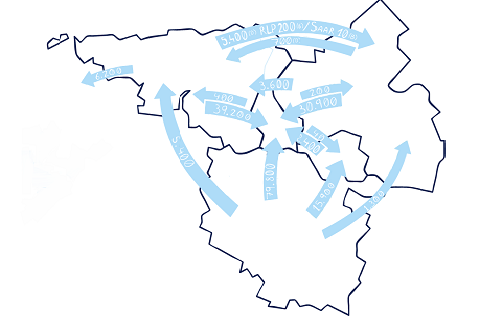
\includegraphics{"~/Documents/covid_grande_region/paper/figs/commuters.png"}
  \caption{The daily commuters in the Greater Region. Luxembourg absorbs the vast majority. (Source: Bienvenue dans la Grande Région, 2018)}
  \label{commuters}
\end{figure}

Figure \ref{commuters} show a map of the Greater Region with the flows
of daily commuters between its constituent regions. Every day, according
to this map from 2018, more than 150000 commuters go to Luxembourg to
work. In 2019, it was reported that this number reached
200000.\footnote{\url{https://paperjam.lu/article/plus-200-000-frontaliers-sur-m}}

The approach I will be using in this paper is thus as follows: I will
train a machine learning model to predict the spread of COVID-19 in
Luxembourg using openly available data on the weekly positive cases of
COVID-19. However, because of the very tight economic and social
integration of Luxembourg to its neighbours I will use as features
weekly positive cases in the border regions as well as Google Mobility
data\footnote{\url{https://www.google.com/covid19/mobility/}} for
Luxembourg to proxy for hard, and soft, lockdowns. I will show that lags
of weekly cases in the neighbouring regions predict cases for
Luxembourg. The end goal however, is \emph{not} to build a model to
predict how many weekly positive cases will be detected in Luxembourg.
This would be a fools errand; in order to predict the future, the future
has to look like the past, but in the case of this pandemic there is
absolutely no guarantee that the future will look like the past, and
there are many reasons for this. First of all, people are constantly
adapting their behaviour, and public health policies are also constantly
being tuned, and getting sometimes more restrictive, sometimes more
relaxed. Secondly, vaccines have started being administrated and it
would be impossible to predict the effect on weekly positive cases using
the approach I'm using. Finally, there's also the threat of the
variants. Here again, it is impossible to predict which new variants
could arise and how much more contagious -and deadly- these could be. So
then, why bother with this paper? The end goal is not prediction, but
explainability. Once the model is trained, I will use explainability
methods to show which variables, and their interaction with each other,
predict positive cases for Luxembourg. This will be a clear illustration
of the hypothesis that I posited at the beginning; that a landlocked
country like Luxembourg which is very tightly economically and socially
integrated with its neighbours cannot fight a pandemic on its own, but
must cooperate with its neighbours. This argument can also be applied to
any other country in the same situation as Luxembourg or even to the
constituent states of a federal nation. Unfortunately, the virus does
not respect the borders of sovereign nations.

\hypertarget{the-covid-19-pandemic-in-the-greater-region}{%
\section{The COVID-19 pandemic in the Greater
Region}\label{the-covid-19-pandemic-in-the-greater-region}}

COVID-19 started to spread in the Greater Region around end of February.
Two french \emph{départements}, the \emph{Bas-Rhin} and the
\emph{Haut-Rhin}, which together form the historical region of Alsace,
were hit very hard. A religious gathering in the \emph{Haut-Rhin}, with
more than 2000 worshipers is the very likely start of the spread in
Alsace, and then to the neighbouring Lorraine administrative region.
Alsace is part of the \emph{Grand Est} region, as is Lorraine. Two
\emph{départements} of \emph{Lorraine} are part of the Greater Region,
and the disease spread there quickly as well.

In Luxembourg, the first identified case was announced during a press
conference on the 29th of February 2020. However, in the publicly
available data, cases start on the week of the 16th. This was never, as
far as I know, explained. However, in August 2020 it was announced that
positive cases detected among non-residents would not be counted
anymore. The only logical conclusion is that the first cases, up until
the 16th of March, were of non-residents.

\begin{Shaded}
\begin{Highlighting}[]
\FunctionTok{tar\_read}\NormalTok{(epid\_curves)}
\end{Highlighting}
\end{Shaded}

\begin{figure}
\centering
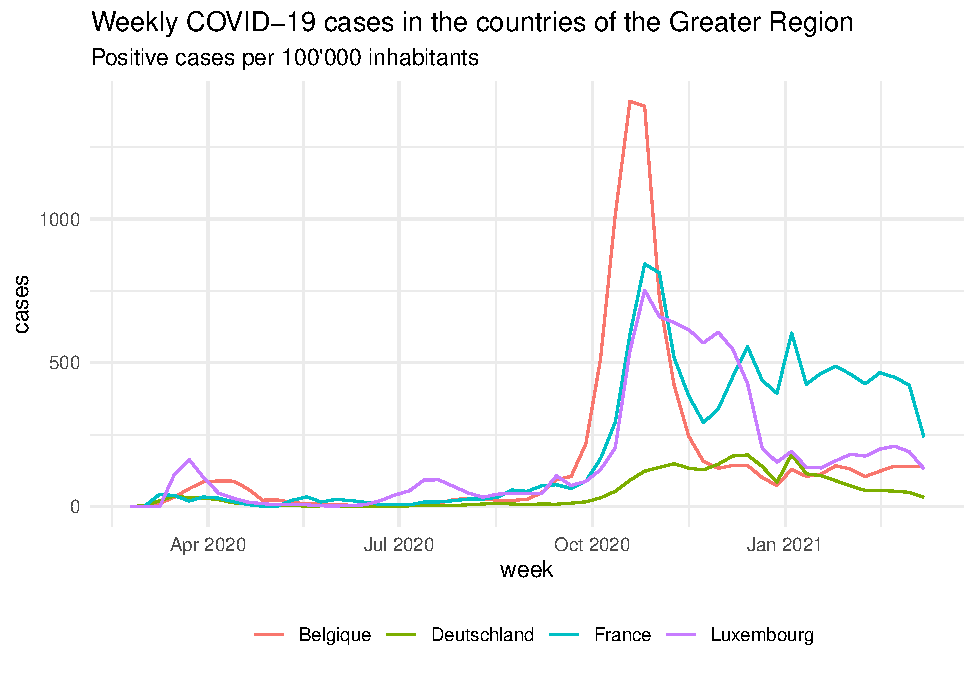
\includegraphics{paper_files/figure-latex/epid_curves-1.pdf}
\caption{Test}
\end{figure}

In Figure @ref(fig:epid\_curves)

\begin{Shaded}
\begin{Highlighting}[]
\FunctionTok{tar\_read}\NormalTok{(epidem\_map)}\SpecialCharTok{$}\NormalTok{map\_first\_wave}
\end{Highlighting}
\end{Shaded}

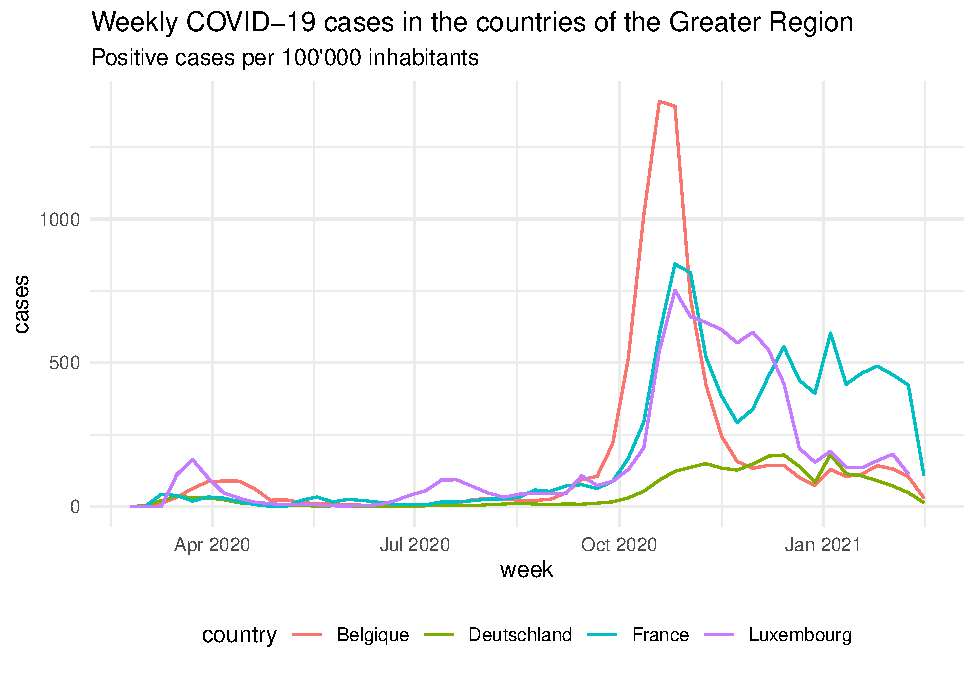
\includegraphics[width=1\linewidth]{paper_files/figure-latex/unnamed-chunk-1-1}

\begin{Shaded}
\begin{Highlighting}[]
\FunctionTok{tar\_read}\NormalTok{(epidem\_map)}\SpecialCharTok{$}\NormalTok{map\_second\_wave}
\end{Highlighting}
\end{Shaded}

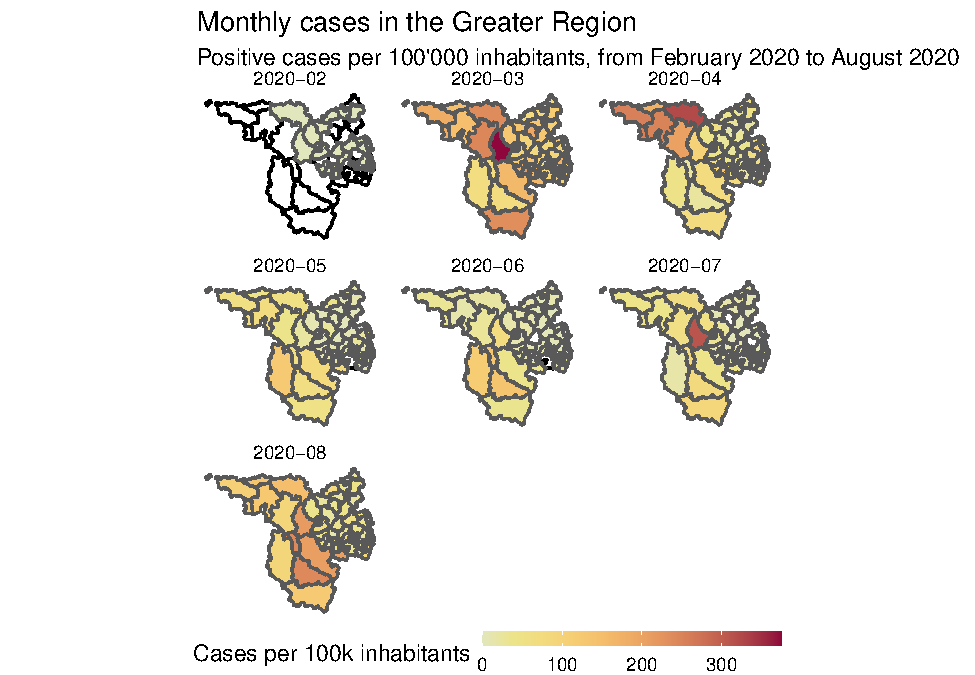
\includegraphics[width=1\linewidth]{paper_files/figure-latex/unnamed-chunk-2-1}

\hypertarget{the-data-used}{%
\section{The data used}\label{the-data-used}}

Data on positive cases from the regions of the Greater Region was
collected through each of the countries' open data portal. The levels of
detail were heterogeneous, with Belgium and Germany providing a high
level of detail (daily cases by sex, age group, Province in the case of
Belgium, and Land- and Stadtkreise in the case of Germany), followed by
France (daily cases by department and age group), with Luxembourg
providing the least amount of details; only daily cases at the national
level. In order to simplify the process of getting the data from all
these sources, we wrote an R package called
\texttt{\{covidGrandeRegion\}} which can be found on the following
\href{https://github.com/b-rodrigues/covidGrandeRegion}{github
repository}. This R package provides several functions to download daily
or weekly data, either for one single country or for the whole of the
Greater Region as well as a function to call an interactive map of the
region with a timeline, making it easy to visualise the spread of the
disease through the region. It is also possible to normalize the data by
dividing the daily or weekly cases by the size of the population in each
sub-region. Another variable that was included comes from the
\href{https://www.google.com/covid19/mobility/}{Google Mobility
website}. This data shows on a daily basis how communities move since
the start of the pandemic. This data is used here as proxy for
lockdowns. The plot below shows the daily percentage change in time
spent at home in Luxembourg:

\begin{Shaded}
\begin{Highlighting}[]
\FunctionTok{tar\_read}\NormalTok{(plot\_mobility)}
\end{Highlighting}
\end{Shaded}

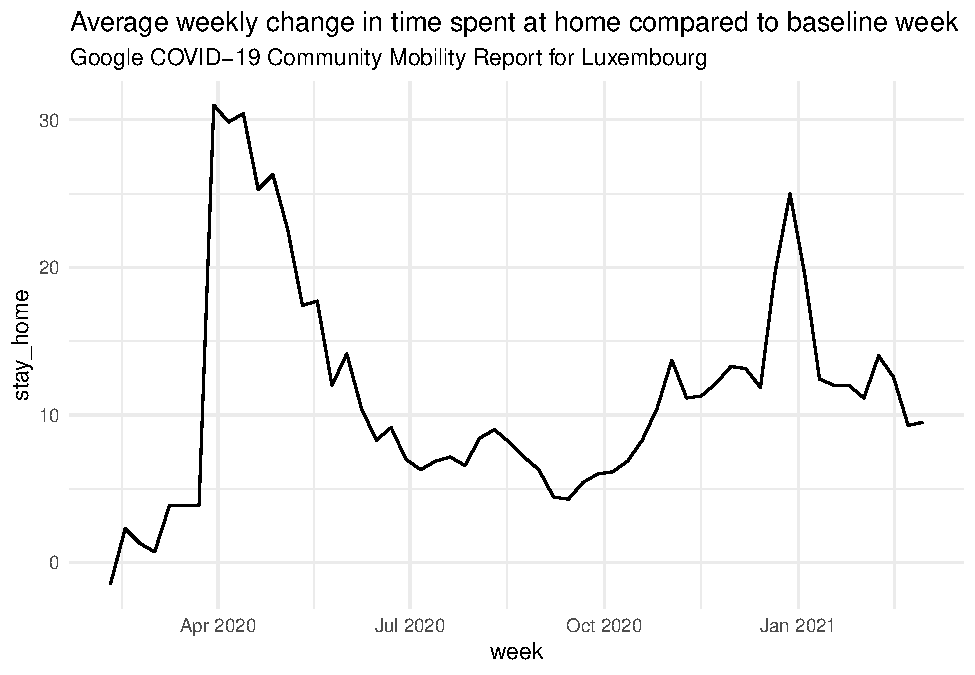
\includegraphics{paper_files/figure-latex/unnamed-chunk-3-1.pdf}

The hard lockdown from March and April can be clearly seen in the data.
Weekly positive cases where divided by the population size in each
region and all the variable were lagged up to four times. The goal of
lagging these variables is to see if cases that were detected in
neighbouring countries in the past 4 weeks have predictive power. The
same was done with the mobility variable (time spent at home in
Luxembourg). The following table shows the structure of data used in
this study:

\begin{Shaded}
\begin{Highlighting}[]
\NormalTok{print\_data }\OtherTok{\textless{}{-}} \FunctionTok{tar\_read}\NormalTok{(data\_for\_model) }\SpecialCharTok{\%\textgreater{}\%}
  \FunctionTok{mutate}\NormalTok{(}\FunctionTok{across}\NormalTok{(}\FunctionTok{where}\NormalTok{(is.numeric), }\SpecialCharTok{\textasciitilde{}}\FunctionTok{round}\NormalTok{(., }\DecValTok{0}\NormalTok{))) }\SpecialCharTok{\%\textgreater{}\%}
  \FunctionTok{t}\NormalTok{() }\SpecialCharTok{\%\textgreater{}\%}
  \FunctionTok{as.data.frame}\NormalTok{() }\SpecialCharTok{\%\textgreater{}\%}
\NormalTok{  tibble}\SpecialCharTok{::}\FunctionTok{rownames\_to\_column}\NormalTok{(}\AttributeTok{var=}\StringTok{"Variable names"}\NormalTok{) }\SpecialCharTok{\%\textgreater{}\%}
  \FunctionTok{select}\NormalTok{(}\FunctionTok{seq}\NormalTok{(}\DecValTok{1}\NormalTok{, }\DecValTok{6}\NormalTok{)) }\SpecialCharTok{\%\textgreater{}\%}
  \FunctionTok{unite}\NormalTok{(}\StringTok{"First 5 observations"}\NormalTok{, }\DecValTok{2}\SpecialCharTok{:}\DecValTok{6}\NormalTok{, }\AttributeTok{sep =} \StringTok{", "}\NormalTok{) }

\FunctionTok{kbl}\NormalTok{(print\_data, }\AttributeTok{booktabs =} \ConstantTok{TRUE}\NormalTok{, }\AttributeTok{position =} \StringTok{"center"}\NormalTok{)}
\end{Highlighting}
\end{Shaded}

\begin{tabular}[t]{ll}
\toprule
Variable names & First 5 observations\\
\midrule
week & 2020-02-24, 2020-03-02, 2020-03-09, 2020-03-16, 2020-03-23\\
Luxembourg & 0,   0,   0, 112, 164\\
lag\_Belgique\_01 & 0,    0,    3,   11,   33\\
lag\_Belgique\_02 & 0,    0,    0,    3,   11\\
lag\_Belgique\_03 & 0,    0,    0,    0,    3\\
\addlinespace
lag\_Belgique\_04 & 0,    0,    0,    0,    0\\
lag\_Deutschland\_01 & 0,   1,   3,  21,  37\\
lag\_Deutschland\_02 & 0,   0,   1,   3,  21\\
lag\_Deutschland\_03 & 0,   0,   0,   1,   3\\
lag\_Deutschland\_04 & 0,   0,   0,   0,   1\\
\addlinespace
lag\_France\_01 & 0,   0,   2,  43,  39\\
lag\_France\_02 & 0,   0,   0,   2,  43\\
lag\_France\_03 & 0,   0,   0,   0,   2\\
lag\_France\_04 & 0,   0,   0,   0,   0\\
lag\_stay\_home\_01 & 0,  1,  1,  4,  4\\
\addlinespace
lag\_stay\_home\_02 & 0,  0,  1,  1,  4\\
lag\_stay\_home\_03 & 0,  0,  0,  1,  1\\
lag\_stay\_home\_04 & 0,  0,  0,  0,  1\\
\bottomrule
\end{tabular}

\texttt{Luxembourg} is the target variable.

\begin{Shaded}
\begin{Highlighting}[]
\FunctionTok{tar\_read}\NormalTok{(cv\_plan)}
\end{Highlighting}
\end{Shaded}

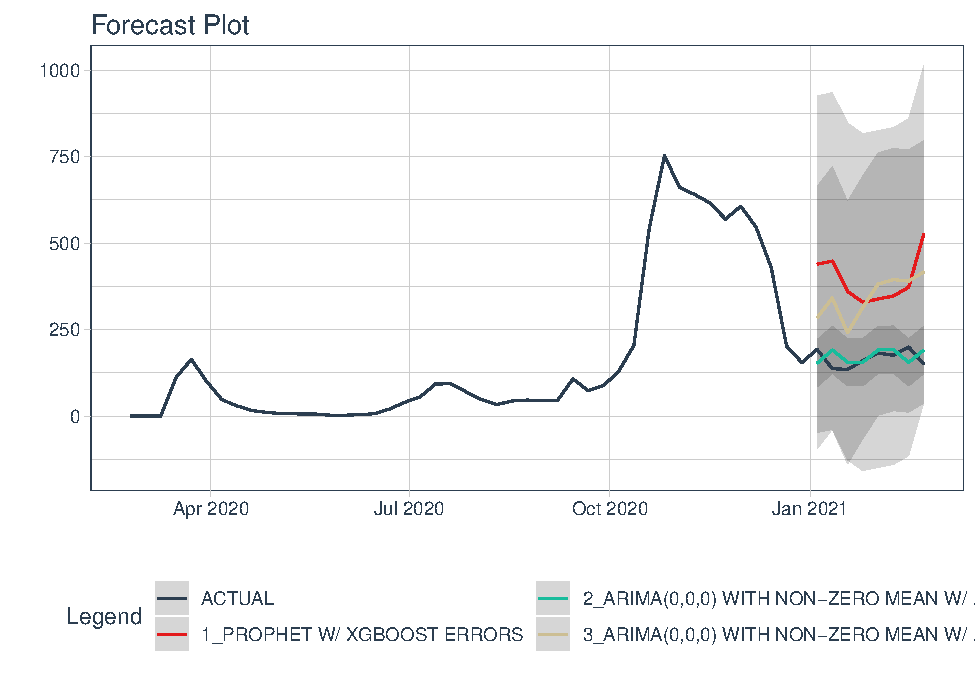
\includegraphics{paper_files/figure-latex/unnamed-chunk-5-1.pdf}

\begin{Shaded}
\begin{Highlighting}[]
\FunctionTok{tar\_read}\NormalTok{(forecast\_plot)}
\end{Highlighting}
\end{Shaded}

\begin{verbatim}
## Warning in max(ids, na.rm = TRUE): no non-missing arguments to max; returning
## -Inf
\end{verbatim}

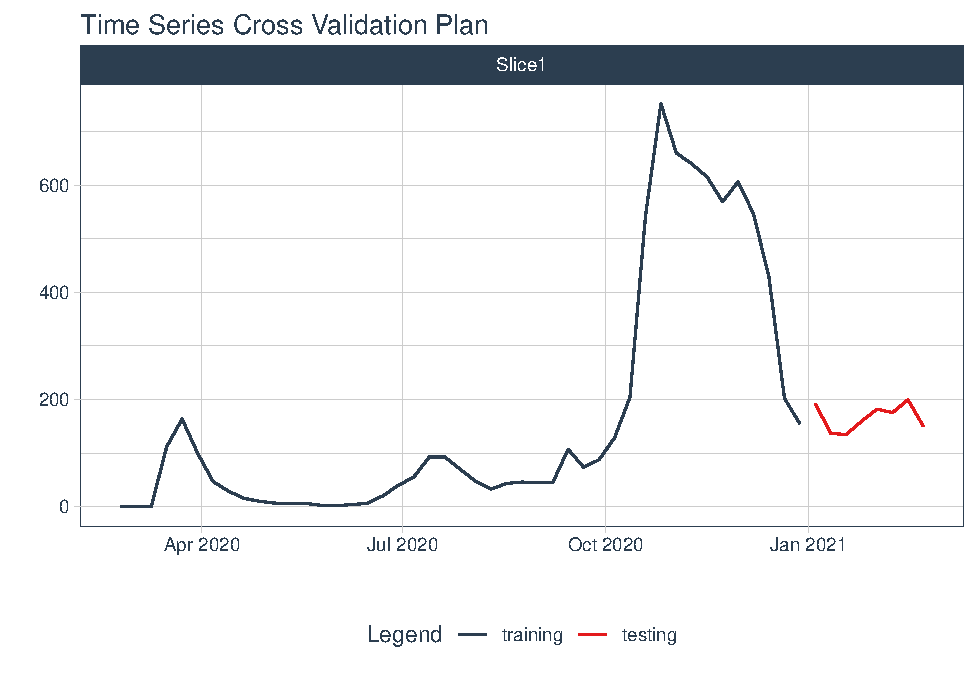
\includegraphics{paper_files/figure-latex/unnamed-chunk-6-1.pdf}

\begin{Shaded}
\begin{Highlighting}[]
\FunctionTok{tar\_read}\NormalTok{(plot\_var\_imp)}
\end{Highlighting}
\end{Shaded}

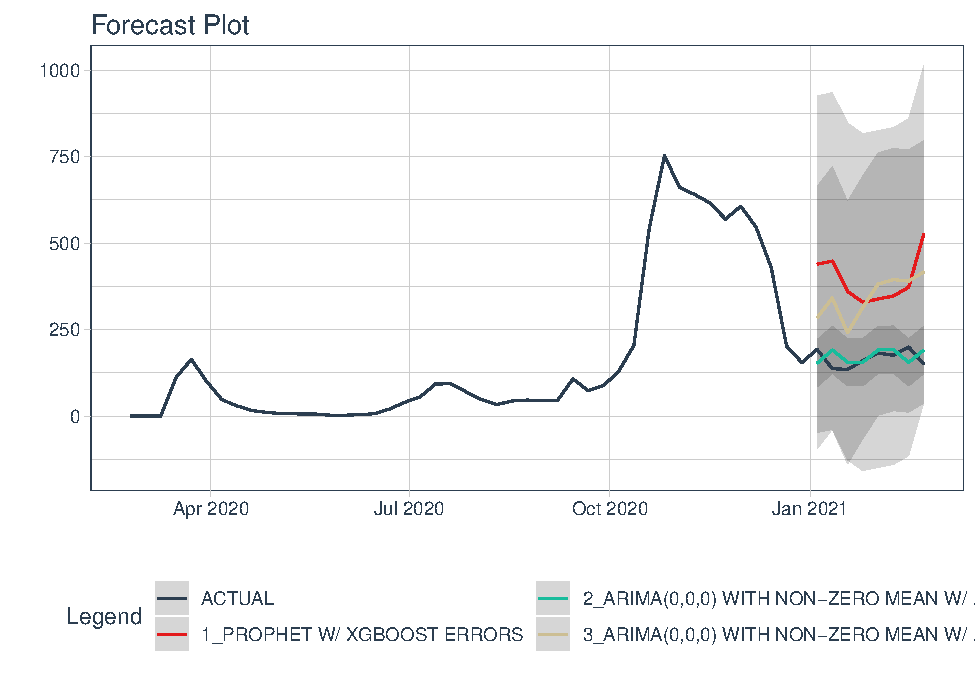
\includegraphics{paper_files/figure-latex/unnamed-chunk-7-1.pdf}

\begin{Shaded}
\begin{Highlighting}[]
\FunctionTok{tar\_read}\NormalTok{(plot\_var\_resp)}
\end{Highlighting}
\end{Shaded}

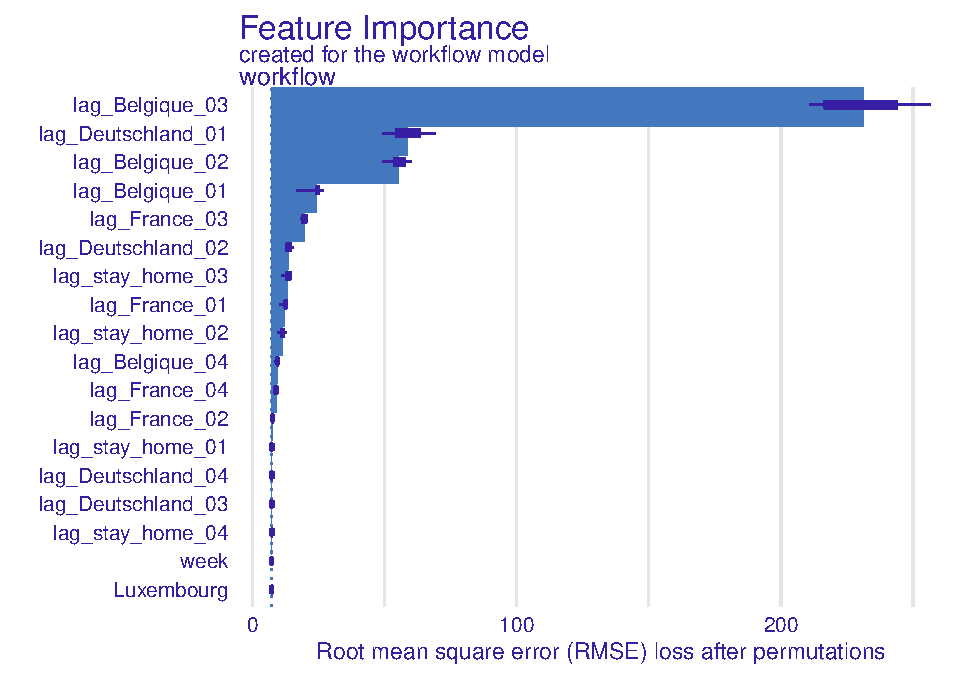
\includegraphics{paper_files/figure-latex/unnamed-chunk-8-1.pdf}

\begin{Shaded}
\begin{Highlighting}[]
\FunctionTok{tar\_read}\NormalTok{(plot\_pred\_contributions)}
\end{Highlighting}
\end{Shaded}

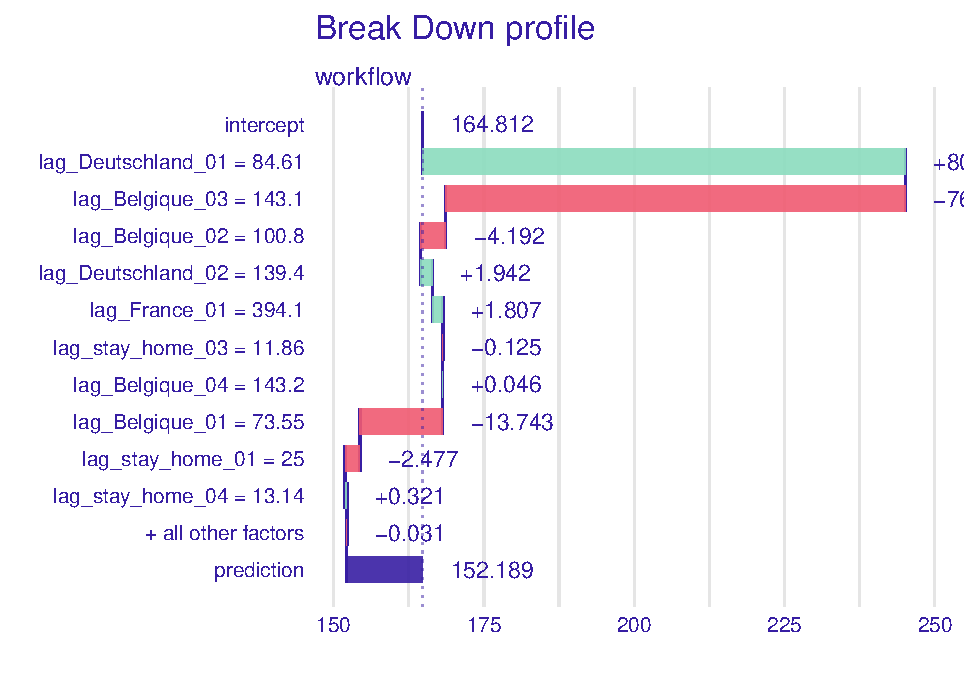
\includegraphics{paper_files/figure-latex/unnamed-chunk-9-1.pdf}

\hypertarget{appendix}{%
\section{Appendix}\label{appendix}}

\bibliographystyle{unsrt}
\bibliography{bibliography.bib}


\end{document}
